\documentclass[a4paper,12pt]{report}
\usepackage{unifrsr}
\usepackage{hsc_texstyle}
\usepackage[style=alphabetic, backend=bibtex]{biblatex}
\addbibresource{references.bib}

\begin{document}
	\seminartitle{Human Smart Cities Seminar} % The title of the seminar

	\title{Wisdom of the Crowds \\ Can Crowd-Sourcing coexist with today’s Data Security Regulations?} % The title of your project

	\author{Pascal Gerig (16-104-721)\thanks{\email{pascal.gerig@students.unibe.ch}, University of Bern}
   		\and Lorenzo Wipfli  (13-933-262)\thanks{\email{lorenzo.wipfli@students.unibe.ch}, University of Bern}
   		\and Marcel Zauder  (16-124-836)\thanks{\email{marcel.zauder@students.unibe.ch}, University of Bern}
   	}	% Note: XX-XXX-XXX is the student's matriculation number
   	% The author(s), separated by \and

	\supervisor{Prof. Edy Portmann} % Name of the supervisor

	\assistant{Moreno Colombo \and Jhonny Pincay} %Name of the assistant(s)

	\date{\today} % Note: if this is left out, today's date will be used, this is the submission date!

	\maketitle

	\begin{abstract}
		This package, \textsf{unifrsr}, allows the easy creation of seminar
		reports using standard \LaTeX. It should be the last
		package loaded, to ensure that nothing overrides the page layout.

		Note that utility commands are available: 
		\begin{itemize}
			\item \verb+\seminartitle+ which specifies, optionally, the title of the seminar the report is being written for
			\item \verb+\supervisor+ which specifies the name of the professor supervisor of the project
			\item \verb+\assistant+ which specifies, optionally, the name of the assistants of the seminar, separated by the command \verb+\and+
		\end{itemize}

		\keywords{Seminar report, Human-IST Research Institute}
	\end{abstract}

	\tableofcontents

	\chapter{Introduction}
		This is an example of a section. As you see, it is just a standard {\LaTeX} section. Here is a footnote%
		\footnote{This is a footnote}.

		\section{Background and Motivation}
		\startsection
			It's all standard \LaTeX, as you can see. This is a very nice paper:
			\nocite{*}
		\closesection
		
	\chapter{General Data Protection Regulation}
	\chaptermark{GDPR}
	The General Data Protection Regulation, referred to as GDPR, is in effect across the European Union from May 25, 2018.
	The Regulation is directly applicable to processing of personal data in the European Union and data collected from its data subjects.
	One central aspect of the regulation is, that it inludes a significant escalation in potential penalties (up to 4\% of the global revenue).
	Figure \ref{fig:enforcement_tracker} shows how enforcement activities increase from commencement until October 2021.
	For instance, Amazon was fined 746 million \texteuro \ in July 2021 \cite{EnforcementTracker}
	\begin{figure}
		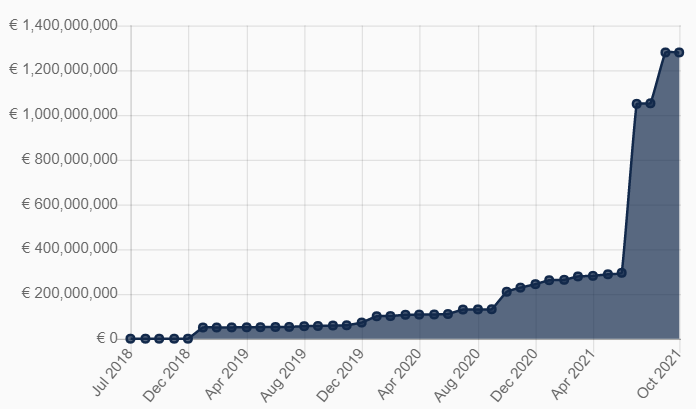
\includegraphics{EnforcementTracker_21-10-12.PNG}
		\caption{Enforcement activities \cite{EnforcementTracker}}
		\label{fig:enforcement_tracker}
	\end{figure}
	
	\section{Core Concepts}
	\startsection
	GDPR defines certain core concepts which are important for the further understanding of the regulation.\\
	\textbf{Personal data} is any information relating to an identified or identifieable natural person.
	There are three subtypes of interest to personal data. 
	First of, \textbf{sensible data} is defined as personal data that is revealing race, ethnic origin, political opinions, religious or philosophical beliefs, trade union membership, health, sex life and sexual orientation, genetic data or biometric data.
	Next, there is data relating to \textbf{criminal offences} and convictions.
	Finally, \textbf{health data} is personal data relating to physical or mental health of an individual, including the provision of healt care services, which reveal information about his or her health status.\\
	\textbf{Pseudonymization} is the processing of personal data in such a manner that the personal data can no longer be attributed to a specific data subject without the use of additional information, provided that such additional information is kept separately and is subject to technical and organisational measures to ensure that the personal data are not attributed to an identified or identifieable natural person.
	\textbf{Anonymization} eliminates personal data so that data subjects can no longer be identified. 
	Anonymized data is excluded from GDPR altogether because anonymized data is no longer personal data.
	\textbf{Data processing} means any operation or set of operations performed upon personal data or sets of personal data, whether or not by automated means, such as collection, recording, organisation, structuring, storage, adaptation or alternation, retrieval, consultation, use, disclosure by transmission, dissemination or otherwise making available, alignment or combination, restriction, erasure or destruction.
	\closesection

	\section{Data Processing Entities}
	\startsection
	The GDPR defines different entities responsible for data processing. These entities have different responsibilites.
	Namely there are the following:
	\begin{enumerate}[]
		\item The Data Controller (Art. 24 \cite{EUdataregulations2018})
		determines the purpose and means of the personal data processing.
		In general, controllers bear primary responsibility for ensuring that processing activities are compliant with the regulation.
		\item The Data Processor (Art. 28 \cite{EUdataregulations2018})
		acts on the conroller's behalf. 
		There is a binding written agreement between the two entities. 
		The controller must ensure the processor's compliance with GDPR.
		\item Joint Controller (Art. 26 \cite{EUdataregulations2018}) is a Data Controller, containing multiple entities.
		Given such a Scenario, the different entities must have an agreement on their respective responsibilites.
	\end{enumerate}
	\closesection

	\section{Data subject rights}
	\startsection
	A identified or identifiable natural person, subject to it's data being processed by a controller, is called a \textbf{data subject}.
	Each data subject has a set of rights under GDPR:
	\begin{enumerate}[]
		\item Right of access (Art. 15)
		\item Right to rectification (Art. 16)
		\item Right to erasure (Art. 17)
		\item Right to restriction (Art. 18)
		\item Right to data portability (Art. 20)
		\item Right to object (Art. 21)
		\item Right not to be subject to decisions based solely on automated processing which produces legal or similarly significant effects (Art. 22)
	\end{enumerate}
	\closesection

	\section{Consent and Privacy Policy}
	\startsection
	bla
	\closesection

	\section{Sanctions}
	\startsection
	bla
	\closesection

	\section{Miscellaneous}
	\startsection
	bla
	\closesection
	
	\chapter{Crowd-Sourcing Methods}
	\startsection
	\closesection
	
	\chapter{Related Work \cite{LanierWeylBlueprint}}
	\startsection
	\closesection


	\newpage
	\addcontentsline{toc}{chapter}{Bibliography}
	\printbibliography
\end{document}
